\section{Методика~использования\\ разработанного приложения}
\label{sec:usage}

Программное средство представляет из себя библиотеку, написанную на языке С++. Использование симулятора возможно в рамках драйвера. Драйвер должен создать объект класса MemorySystem, инициализировать его и зарегистрировать функции обратной связи. Организовав цикл, драйвер должен отсчитывать такты для симулятора, вызывая на каждой итерации метод update класса MemorySystem. Команды чтения и записи отправляются системе памяти через метод addTransaction.

Объект класса MemorySystem инициализируется значениями:

\begin{enumerate}
\item deviceIniFilename -- путь к файлу конфигурации памяти;
\item systemIniFilename -- путь к файлу инициализации системы;
\item traceFilename -- путь к файлу регистрации, если он не задан, то все сообщения выводятся на консоль;
\item megsOfMemory -- объём симулируемой памяти в мегабайтах;
\item fualtFilePath -- путь к файлу неисправностей;
\item marchTest -- название маршевого теста, который будет запускаться для выявления неисправностей;
\item refreshPeriodShift -- количество тактов, на которое будет сдвинут период обновления памяти.
\end{enumerate}

Функции обратной связи полчают уведомления о выполнении транзакций. Необходимо зарегистрировать две функции, одна из которых будет получать уведомления о выполнении операции записи в память, а вторая результат операции чтения. Сигнатуры функций обратной связи представлены в листинге \ref{lst:udage:callbacks}.

\begin{lstlisting}[style=cplusplusstyle, caption={Сигнатуры функций обратного вызова}, label=lst:udage:callbacks]
void read_complete(uint64_t address, uint16_t data, size_t);
void write_complete(unsigned id, uint64_t address, uint64_t cycle);
\end{lstlisting}

Создание объекта MemorySystem и регистрация функций обратного вызова представлена в листинге \ref{lst:udage:callback_register}.

\begin{lstlisting}[style=cplusplusstyle, caption={Инициализация системы и регистрация функций обратного вызова}, label=lst:udage:callback_register]
string systemIniFilename = "system.ini";
string deviceIniFilename = "ini/DDR2_micron_1Mb.ini";
unsigned megsOfMemory = 1;

memory = new MemorySystem(0, deviceIniFilename, systemIniFilename, "", "SimulationResults.txt", megsOfMemory, 0, "MATS++", "faults.csv");

ReadDataCB *read_cb = new Callback<TestingSystem, void, uint64_t, uint16_t, size_t>(this, &TestingSystem::read_complete);
TransactionCompleteCB *write_cb = new Callback<TestingSystem, void, unsigned, uint64_t, uint64_t>(this, &TestingSystem::write_complete);
memory->RegisterCallbacks(read_cb, write_cb, 0);
\end{lstlisting}

Файл конфигурации памяти имеет расширение ini и состоит из следующих параметров:
\begin{enumerate}
\item NUM\_BANKS -- количество банков в одном ранке;
\item NUM\_ROWS -- количество рядов в матрице запоминающих элементов банка;
\item NUM\_COLS -- количество колонок в матрице запоминающих элементов банка;
\item DEVICE\_WIDTH -- объем одной ячейки матрицы запоминающих элементов банка;
\item REFRESH\_PERIOD -- время в наносекундах, через которое память переходит в режим обновления, причем один цикл работы системы длится условно три наносекунды.
\end{enumerate}

Остальные параметры являются специфическими настройками временных характеристик конкретного вида памяти.

Файл инициализации системы имеет расширение ini и состоит из следующих параметров:
\begin{enumerate}
\item TRANS\_QUEUE\_DEPTH -- длина очереди транзакций;
\item CMD\_QUEUE\_DEPTH -- длина очереди команд;
\item DEBUG\_TRANS\_Q -- флаг, регулирующий трансляцию пакетов, поступающих в очередь транзакций;  
\item DEBUG\_CMD\_Q -- флаг, регулирующий трансляцию пакетов, поступающих в очередь команд;  
\item DEBUG\_ADDR\_MAP -- флаг, регулирующий трансляцию сообщений от дешифратора адресов; 
\item DEBUG\_BUS -- флаг, регулирующий трансляцию пакетов, проходящих по шине данных; 
\item DEBUG\_BANKSTATE -- флаг, регулирующий трансляцию состояния банков памяти.
\end{enumerate}

Файл неисправностей имеет расширение csv. Файл представляет собой текстовой документ, в котором сохранена табличная информация. Все колонки таблицы разделены символом табуляции. Всего различается пять колонок. Первая колонка содержит название модели неисправности. Это поле может принимать одно из следующих значений: SAF, TF, AF, CFin, CFid, CFst. Вторая и четвертая колонка содержит адреса ячейки-жертвы и ячейки-агрессора в шестнадцатиричном формате. Третья и пятая колонка содержит значения ячейки-жертвы и ячейки-агрессора в соответствии с моделью неисправности. Для неисправностей типа SAF и TF четвертое поле (адрес ячейки-агрессора) не используется, так же, как и пятое поле (значение ячейки-агрессора). Пример файла, описывающего неисправности, приведён на рисунке \ref{fig:usage:faults_file}.

\begin{figure}[ht]
\centering
  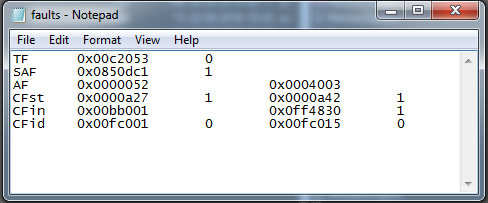
\includegraphics[scale=0.8]{a_faults_file.png}  
  \caption{Файл описания неисправностей памяти}
  \label{fig:usage:faults_file}
\end{figure}

На рисунке \ref{fig:usage:console_read_write} приведён скриншот работы программы при исправной памяти. Операции четния и записи транслируются с двух сторон: от драйвера и от контроллера памяти.

\begin{figure}[ht]
\centering
  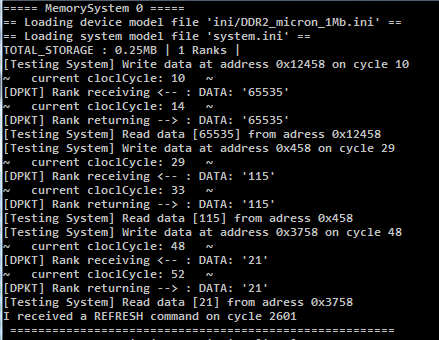
\includegraphics[scale=1]{a_console_read_write.png}  
  \caption{Работа симулятора при исправном устройстве памяти}
  \label{fig:usage:console_read_write}
\end{figure}

При сдвинутом периоде обновления памяти произвольные ячейки ОЗУ теряют свой заряд. Чем больше времени прошло с момента не наступившего сигнала Refresh, тем больше ячеек повредится. Эти изменения в памяти засекает адаптивный сигнатурный анализатор, который при наступлении периода обновления памяти вычисляет рабочую сигнатуру. Пример работы симулятора со сдвинутым периодом обновления приведен на рисунке \ref{fig:usage:console_discharge}.

\begin{figure}[ht]
\centering
  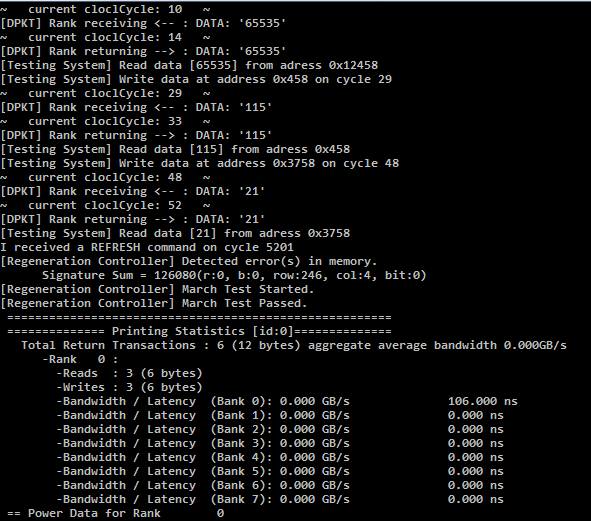
\includegraphics[scale=1]{a_console_discharge.png}  
  \caption{Работа симулятора при сдвинутом периоде обновления памяти}
  \label{fig:usage:console_discharge}
\end{figure}

На рисунке \ref{fig:usage:console_discharge} видно, что АСА засек ошибки в памяти, т.к. эталонная и рабочая сигнатуры не совпали, и запустил маршевый тест для выявления неисправностей. Разрядка конденсаторов динамического ОЗУ является ошибкой, а не функциональной неисправностью, а потому маршевый тест ничего не обнаружил. 

На рисунке \ref{fig:usage:console_march} показана работа симулятора памяти при наличии неисправностей. В файле описания неисправностей записано две модели неисправностей: SAF и CFst. Ячейка-жертва находится по адресу 0x27, т.е. 0-ой ранк, 0-ой банк, 0-ая строка, 2-ая колонка и 7-ой бит. Эта ячейка не может поменять значение логической единицы на логический ноль, если ячейка-агрессор, которая находится по адресу 0x42, содержит логический ноль. 

\begin{figure}[ht]
\centering
  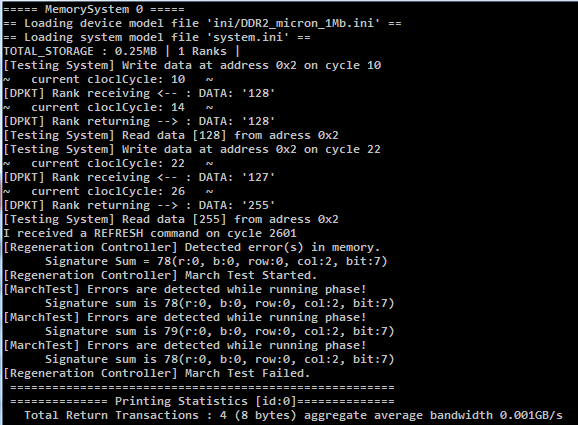
\includegraphics[scale=1]{a_console_march.png}  
  \caption{Работа симулятора при наличии функциональных неисправностей}
  \label{fig:usage:console_march}
\end{figure}

На рисунке \ref{fig:usage:console_march} отображено, что в начале в ячейку по адресу 0x2 (0-ой ранк, 0-ой банк, 0-ая строка, 2-ая колонка) было записано значение 128, что означает запись логической единицы в 7-ой бит слова. Операция чтения по этому же адресу подтверждает, что ячейка хранит это значение. Но при попытке записать значение 127 в ячейку памяти, что означает запись в биты с 0-го по 6-ой значения логической единицы, а в 7-ой бит логического нуля, в реальности сохраняется значение 255, т.е. 7-ой бит не смог поменять своё состояние из-за неисправности. АСА засек неполадку и запустил маршевый тест March C-, который в свою очередь обнаружил неисправность в памяти.